\chapter{Review of papers}

\myminitoc

\sect{Sinkhorn Distances: Lightspeed Computation of Optimal Transport \cite{Cut}}

In this paper written in 2013, Cuturi proposed one of the most currently used algorithm to compute Wasserstein distances. He smoothed the classic optimal transport problem thanks to an entropy-regularization and it leads to a new distance which has a faster solver. He also showed that using regularization gives better results on MNIST classification problem than using the classic Wasserstein distance or obviously the Euclidean distance. This paper is part of the search for adequate and easily computable distances in machine learning. Wasserstein distance is better than Euclidean distance in many cases of machine learning but because the complexity to compute it is $\mathcal{O}(n^3 \log n)$ for $n$ the size of the data, Wasserstein distance is rarely used. That's why techniques to compute the Wasserstein distance had to be develop.

\paragraph{Idea}
The main ideas of this paper are the use of an entropic-regularization to simplify computation when using Sinkhorn iterative algorithm and the idea of computing the distances between one point and a family of other points in the same time, to use matrix-matrix multiplications instead of matrix-vector multiplications while computing distances between pair of points. Thus the algorithm can be implemented on GPU architectures.

\paragraph{Regularization}
We recall that the goal of the optimal transport problem in the Kantorovich formulation is to find a joint distribution $P \in \R^{n \times n}$ where the marginals equal the two distributions for which we want to compute the distance. That is to say $P \mathbbm{1}_n = a$ and $P^\trans \mathbbm{1}_n = b$ when we compute the distance between $a$ and $b$. We call $U(a, b)$ the set of all possible values for $P$. By denoting the entropy by $H$ we can show that:
$$ H(P) \leqslant H(a) + H(b) $$
And $H(P) = H(a) + H(b)$ when $P = a b^\trans$. We then restrict $P$ to the new set:
$$ U_\alpha(a, b) = \{ P \in U(a, b) \, | \, \text{KL}(P || a b^\trans) \leqslant \alpha \} = \{ P \in U(a, b) \, | \, H(P) \geqslant H(a) + H(b) - \alpha \} $$
Two reasons are given to this restriction. The first one is that it will be easier to compute the distance. The second is that without regularization $P$ has almost $2n-1$ non-zero coefficients. Thus the transport is almost deterministic and it is not natural. That's why smoothing the transport plan with entropic regularization is presented as a good idea. In the paper, it is shown that this restriction induce a new distance:
$$ d_{M, \alpha} = \min_{P \in U_\alpha(a, b)} \langle P, M \rangle $$
Were $M$ is a distance matrix.

\paragraph{Computation}
By duality theory he obtained that to $\alpha$, corresponds a value $\lambda \geqslant 0$ such that the distance $d_{M, \alpha}$ is equal to the distance $d_M^\lambda$ defined by:
$$ d_M^\lambda(a, b) = \langle P^\lambda, M \rangle, \quad \text{where } P^\lambda = \argmin_{P \in U(a, b)} \langle P, M \rangle - \dfrac{1}{\lambda} H(P) $$
Then Cuturi show that this new distance can be computed with a much cheaper cost than the original Wassertein distance $d_M$. In fact the iterative Sinkhorn algorithm presented below converge in few steps to the transport plan $P^\lambda$. The \figurename~\ref{recap1} summarize the relationships between all these distances.

\vspace{3mm}
\begin{algorithm}[H]
	\caption{\textsc{Sinkhorn}$\left( a, \{ b_i \}_{i=1}^N, M, \lambda \right)$}
	$B \gets \left[ b_1, \dots, b_N \right] \in \R^{n \times N}$ \;
	$K \gets \exp \left( \lambda M \right)$ \;
	$u = \left[ u_1, \dots, u_N \right] \gets \mathbbm{1}_{n \times N} \, / \, n$ \;
	\Repeat{convergence of $u$}{
		$u \gets a \, / \, \left( K \left( B \, / \, \left( K^\trans u \right) \right) \right)$ \;
	}
	$v = \left[ v_1, \dots, v_N \right] \gets B \, / \, \left( K^\trans u \right)$ \;
	$P^\lambda_i \gets \text{diag}(u_i) K \text{diag}(v_i)$ \;
	\Return $d = \left[ d_M^\lambda(a, b_1), \dots, d_M^\lambda(a, b_N) \right] = \left[ \left\langle M, P^\lambda_1 \right\rangle, \dots, \left\langle M, P^\lambda_N \right\rangle \right]$
\end{algorithm}
\vspace{3mm}

\begin{figure}
	\centering
	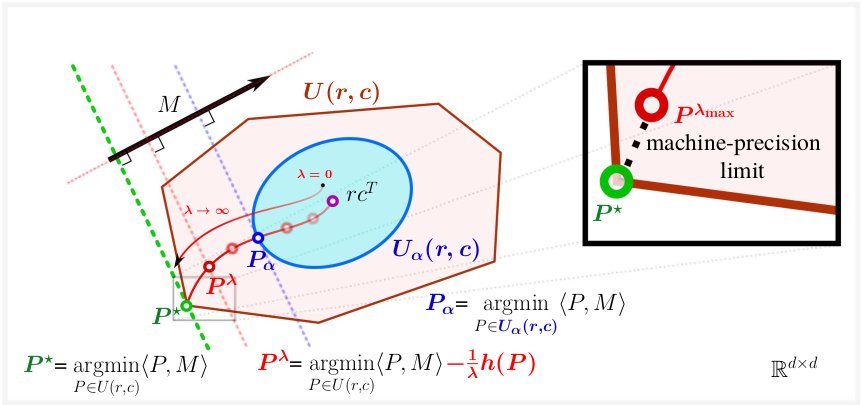
\includegraphics[scale=0.5]{recap1.png}
	\captionsetup{justification=centering}
	\caption{Graphical representation of different distances and their relationships.}
	\label{recap1}
\end{figure}

\paragraph{Results}
The regularized Wasserstein distance is then used in a SVM to classifiy images of the MNIST database. The \figurename~\ref{comp} compare the error on a test set for different distances used in the SVM. The distance EMD is the classical optimal transport. As we can see the regularized version beat all distances. Furthermore he evaluated the execution time by stopping the iterations when $\| d_{i+1} / d_i - 1 \| < 10^{-4}$ where $d_i$ is the distance obtained at the end of the iteration $i$. He gave a comparison between EMD and regularized Wasserstein for different values of $\lambda$ in the \figurename~\ref{comp2}.

\begin{figure}[h]
	\centering
	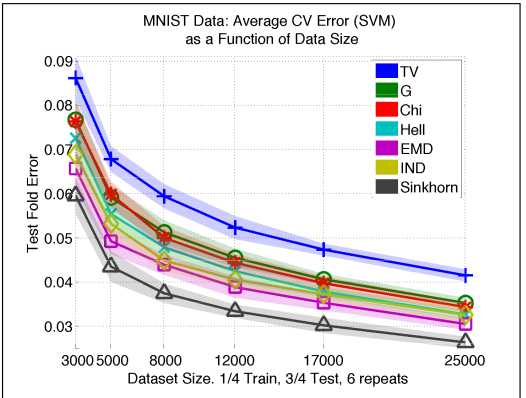
\includegraphics[scale=0.55]{comp.png}
	\caption{Test error for different distances}
	\label{comp}
\end{figure}
\begin{figure}[h]
\centering
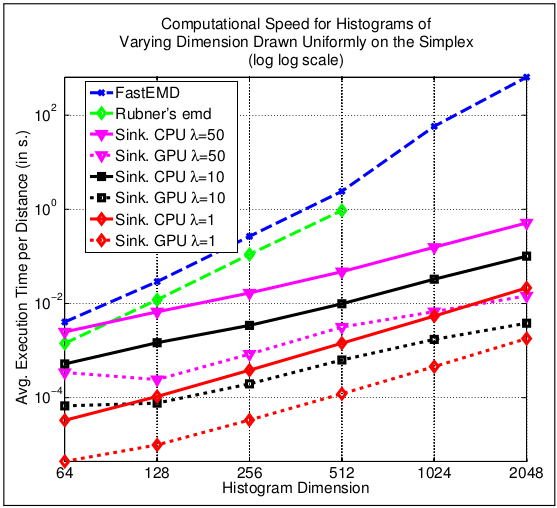
\includegraphics[scale=0.5]{comp2.png}
\caption{Execution time for different distances}
\label{comp2}
\end{figure}

\newpage

\sect{Wasserstein GAN \cite{Arj++}}

This paper proposes a new GAN training algorithm based on Wasserstein distance. When we learn a probability we need to use a divergence between probability distributions. In a first time they show the advantages of the Wasserstein distance over all well-known other divergences on probabilities. Thanks to their WGAN (for Wasserstein GAN), they cure the problem of the need of maintaining a balance between training discriminator and training generator. They also observed that the mode dropping phenomenon is reduced. Furthermore their GAN allows to plot the Wasserstein distance continuously which is very usefull for debugging and to have an estimation of the quality.

\paragraph{Advantage of Wasserstein distance}
They illustrate the interest of Wasserstein distance on the convergence of the probability $\Pp_\theta = g_\theta(Z) = (\theta, Z)$ toward $\Pp_0 = (0, Z)$ for $Z \sim U([0, 1])$ when $\theta$ tends to 0. We have:
\begin{itemize}
	\item $W(\Pp_0, \Pp_\theta) = | \theta |$ where $W$ is the Wasserstein distance.
	\item $JS(\Pp_0, \Pp_\theta) = \left\{ \begin{array}{ll}
			\log 2 & \text{if } \theta \neq 0 \\
			0 & \text{if } \theta = 0
		\end{array} \right.$ where $JS$ is the Jensen-Shannon divergence.
	\item $KL(\Pp_0, \Pp_\theta) = JS(\Pp_\theta, \Pp_0) = \left\{ \begin{array}{ll}
			+ \infty & \text{if } \theta \neq 0 \\
			0 & \text{if } \theta = 0
		\end{array} \right.$ where $KL$ is the Kullback-Leibler divergence.
	\item $\delta(\Pp_0, \Pp_\theta) = \left\{ \begin{array}{ll}
			1 & \text{if } \theta \neq 0 \\
			0 & \text{if } \theta = 0
		\end{array} \right.$ where $\delta$ is the total variation distance defined as \\ $\delta(\Pp_0, \Pp_1) = \sup_{A \in \Sigma} | \Pp_0(A) - \Pp_1(A) |$ with $\Sigma$ the set of all Borel subsets.
\end{itemize}
Thus the Wasserstein distance is the only one for which there is convergence. Then a gradient descent can be applied with the Wasserstein distance but it can't be applied with other divergences. This is a just an example but they also proved the following theorem which shows the continuity under some assumptions:

\PROP{
	Let $\Pp_r$ be a distribution over $\mathcal{X}$ and let $Z$ be a distribution over another space $\mathcal{Z}$ (e.g Gaussian). Let $g : \R^d \times \mathcal{Z} \rightarrow \mathcal{X}$ be a function that will be denoted $g_\theta(z)$ for $g(\theta, z)$. We denote by $\Pp_\theta$ the distribution of $g_\theta(Z)$. Then:
	\begin{itemize}
		\item If $g$ is continuous in $\theta$, so is $W(\Pp_r, \Pp_\theta)$.
		\item If $g$ is locally Lipschitz and satisfies the following regularity assumption: By denoting the local Lipschitz constant $L(\theta, z)$ we have $\E_{z \sim Z} \left[ L(\theta, z) \right] < + \infty$. Then $W(\Pp_r, \Pp_\theta)$ is continuous everywhere and almost differentiable everywhere.
		\item The two previous statements are false for Jensen-Shannon and KL divergences.
	\end{itemize}
}

They also give another theorem that well show that the Wasserstein distance is a very natural divergence for probability distributions:

\PROP{
	Consider a sequence of distributions $(\Pp_n)$ on a compact space $\mathcal{X}$. If $W(\Pp_n, \Pp) \rightarrow 0$ for a certain distribution $\Pp$, then $\Pp_n \xrightarrow{\mathcal{D}} \Pp$ where the limit is in the sense of the convergence in distribution.
}

\paragraph{WGAN}
To construct their GAN they need to compute the gradient of $W(\Pp_r, \Pp_\theta)$ with respect to $\theta$. For that they consider the following dual formulation of the Wasserstein distance:
$$ W(\Pp_r ,\Pp_\theta) = \max_{\| f \|_L \leqslant 1} \E_{x \sim \Pp_r} \left[ f(x) \right] - \E_{x \sim \Pp_\theta} \left[ f(x) \right] $$
Where $\| f \|_L$ denote the Lipshitz coefficient of $f$. If $f$ is the solution to the maximization problem then the gradient is:
$$ \nabla_\theta W(\Pp_r, \Pp_\theta) = - \E_{z \sim Z} \left[ \nabla_\theta f(g_\theta(z)) \right] $$
To find $f$ they train a neural network parameterized with weights $w$ in a compact space $\mathcal{W}$ that lead to a function $f_w$. Then they can backprop $\theta$ using $\E_{z \sim Z} \left[ \nabla_\theta f_w (g_\theta(z)) \right]$.  To have $w$ in a compact space, they use weight clamping. Their algorithm is in the \figurename~\ref{algo}.

\begin{figure}[t]
	\centering
	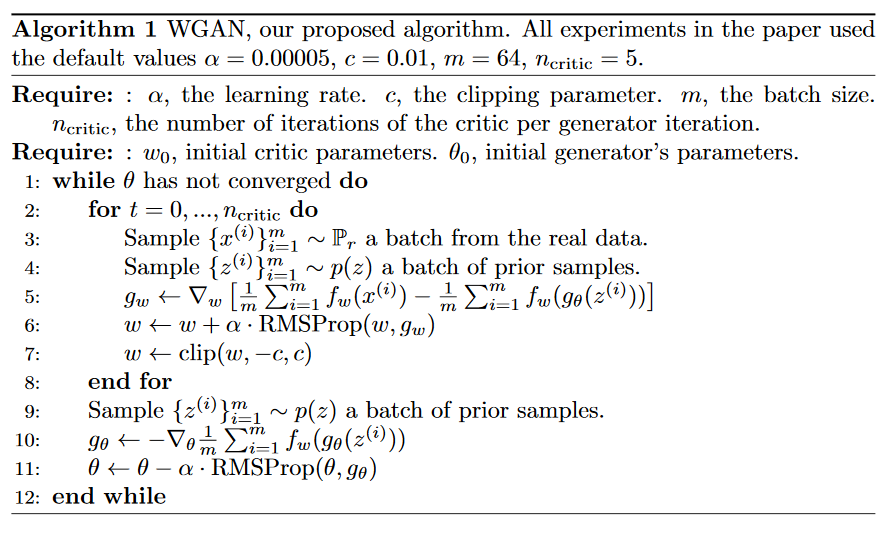
\includegraphics[scale=0.6]{algorithm.png}
	\caption{Algorithm of the WGAN}
	\label{algo}
\end{figure}

\paragraph{results}
First, the authors set up a small experiment to showcase the difference between GAN and WGAN (\figurename~\ref{compa}). There are two 1D Gaussian distributions, blue for real and green for fake. Train a GAN discriminator and WGAN critic to optimality, then plot their values over the space. The red curve is the GAN discriminator output, and the cyan curve is the WGAN critic output.

\begin{figure}[h]
	\centering
	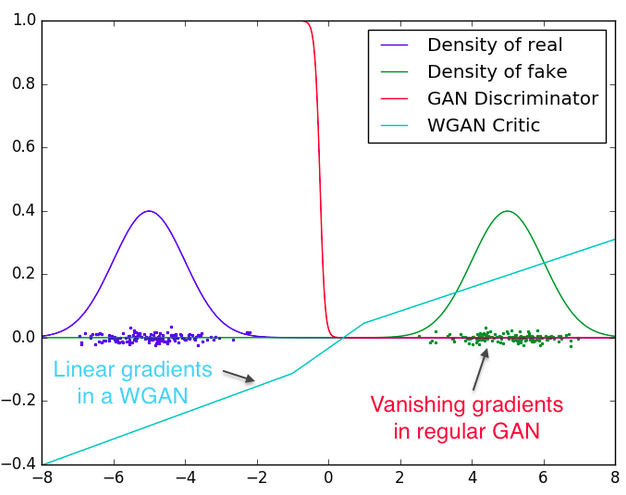
\includegraphics[scale=0.36]{wgan_res.png}
	\caption{Comparison between a GAN discriminator and the WGAN Critic}
	\label{compa}
\end{figure}

Both identify which distribution is real and which is fake, but the GAN discriminator does so in a way that makes gradients vanish over most of the space. In contrast, the weight clamping in WGAN gives a reasonably nice gradient over everything.

Another important point is that the quality of the generation is correlated to Wasserstein estimation as we can see in the \figurename~\ref{meaning}. We  can also see that the training of the critic function $f$ works well as the Wasserstein estimator strictly decrease. The gradient of the loss function is well computed. But this is not a method to compare the quality of different GANs as the estimator is defined with a constant scaling factor depending on the critic's architecture. They finally observed an improvement of the stability. 

\begin{figure}
	\centering
	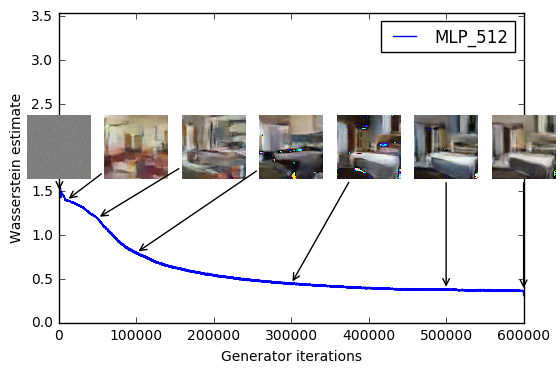
\includegraphics[scale=0.45]{meaning.png}
	\caption{Sample images at different iterations of the training}
	\label{meaning}
\end{figure}

\sect{Convolutional Wasserstein Distances: Efficient Optimal Transportation on Geometric Domains \cite{Goe++}}

Because a single step of Sinkhorn algorithm has a complexity in $\mathcal{O}(n^2)$, computing the Wassertein distance may take a while in many cases. That's why the researchers who write this paper thought about a more effective solution to compute a step. They found a way to use Gaussian convolution with a $\mathcal{O}(n \log n)$ complexity instead of a matrix-vector product. More generally they use a heat kernel. So instead of the convolution it can also be a sparse pre-factored linear system which can be computed in a complexity smaller than $\mathcal{O}(n^2)$. Furthermore by doing this, the convergence is still linear. Of course this can not be applied in all cases of optimal transport, but it can be used on very common geometric domains, like images or meshes. In addition of the computation of Wasserstein distance, they also propose a way to use convolution in the computation of Wasserstein barycentres and Wasserstein propagation.

\paragraph{Using a heat kernel in the entropy-regularization}
We recall what is the entropy-regularized Wasserstein distance between $\mu_0$ and $\mu_1$ on the domain $M$:
$$ W_{2, \gamma}^2(\mu_0, \mu_1) = \inf_{\pi \in \Pi} \left[ \int \int_{M \times M} d(x, y)^2 \pi(x, y) dx dy \, - \, \gamma H(\pi) \right] = \gamma \left[ 1 + \min_{\pi \in \Pi} \text{KL}(\pi | \mathcal{K}_\gamma) \right]$$
Where:
$$ \Pi = \left\{ \pi \in \text{Prob}(M \times M) \, | \, \pi(\cdot, M) = \mu_0, \pi(M, \cdot) = \mu_1 \right\} $$
$$ H(\pi) = - \int \int_{M \times M} \pi(x, y) \ln \pi(x, y) dx dy $$
$$ \mathcal{K}_\gamma = e^{-d(x, y)^2 / \gamma} $$
$$ \text{KL}(\pi | \mathcal{K}) = \int \int_{M \times M} \pi(x, y) \left[ \ln \dfrac{\pi(x, y)}{\mathcal{K}(x, y)} - 1 \right] dx dy $$
This is a strictly convex problem thanks to the entropy. The idea of the paper is to use heat kernel because in some cases, the solution of the diffusion equation can be computed in a effective way. We denote by $\mathcal{H}_t(x, y)$ the diffusion between $x$ and $y$ after a time $t$ in the heat kernel. Just remember that the heat kernel is a solution of the heat equation:
$$ \dfrac{\partial f}{\partial t} = \Delta f $$
One can show the following approximation:
$$ \mathcal{K}_\gamma \approx \mathcal{H}_{\gamma / 2}(x, y) $$
We won't store $\mathcal{H}$ because it could have a space complexity in $\mathcal{O}(n^2)$ and we want a lower complexity. But we generally know a way to apply $\mathcal{H}$ to a vector. In the case of images we apply Gaussian convolution with $\sigma^2 = \gamma$. \\
In the case of triangle meshes we associate a weight to faces proportional to their area. We denote by $a$ the vector of these weights (In images of size $n \times m$ we set $a = 1 / (nm)$). Then we denote by $L$ the cotangent Laplacian and by $D_a$ the diagonal matrix with diagonal $a$. By discretizing the heat equation, we obtain:
$$ w = \mathcal{H}_t(v) \Leftrightarrow \left( D_a + t L \right) w = v $$
The linear system can be solved efficiently by pre-computing a sparse Cholesky factorization.

\paragraph{Algorithm}
With some computations we arrive at:

\vspace{3mm}
\begin{algorithm}[H]
	\caption{\textsc{Convolutional-Sinkhorn}($\mu_0, \mu_1, H_t, a$)}
	$v, w \gets 1$ \;
	\Repeat{convergence of $v, w$}{
		$v \gets \mu_0 \oslash H_t(a \otimes w)$ \;
		$w \gets \mu_1 \oslash H_t(a \otimes v)$ \;
	}
	\Return $2t a^\trans \left[ \left( \mu_0 \otimes \ln v \right) + \left( \mu_1 \otimes \ln w \right) \right]$
\end{algorithm}
\vspace{3mm}

Where $\oslash$ and $\otimes$ denote element-wise operations. As Sinkhorn algorithm we obtain a simple iterative algorithm where, this time, steps can be computed in $\mathcal{O}(n \log n)$ in many cases, where $n$ is the size of the domain $M$.

\paragraph{Barycenter}
An algorithm for computing barycenters is also provided. We won't enter into details but we give their algorithm for computing the barycenter of distributions $\mu_i$ associated with weights $\alpha_i$ for $1 \leqslant i \leqslant k$:

\vspace{3mm}
\begin{algorithm}[H]
	\caption{\textsc{Convolutional-Barycenter}($\{\mu_i\}, \{ \alpha_i \}, H_t, a$)}
	$v_1, \dots, v_k \gets 1$ \;
	$w_1, \dots, w_k \gets 1$ \;
	\Repeat{convergence of $v_i, w_i$}{
		$\mu \gets 1$ \;
		\For{$i = 1, \dots, k$}{
			$w_i \gets \mu_i \oslash H_t(a \otimes v_i)$ \;
			$d_i \gets v_i \otimes H_t(a \otimes w_i)$ \;
			$\mu \gets \mu \otimes d_i^{\alpha_i}$ \;
		}
		\vspace{3mm}
		// Optional \;
		$\mu \gets $ \textsc{Entropic-Sharpening}$\left( \mu, \max_i H(\mu_i) \right)$ \;
		\vspace{3mm}
		\For{$i = 1, \dots, k$}{
			$v_i \gets v_i \otimes \mu \oslash d_i$ \;
		}
	}
	\Return $2t a^\trans \left[ \left( \mu_0 \otimes \ln v \right) + \left( \mu_1 \otimes \ln w \right) \right]$
\end{algorithm}
\vspace{3mm}
Where entropic sharpening allow us to make the entropy of the result $\mu$ smaller than the maximum entropy of all $\mu_i$. To do so if $H(\mu)$ is greater than $\max_i H(\mu_i)$, then we set $\mu$ to $\mu^\beta$ where $\beta$ is such that $H(\mu^\beta) = \max_i H(\mu_i)$. We can find $\beta$ using Newton's method.

\paragraph{Applications}
This has many applications in geometric domains. Applications that are given are:
\begin{itemize}
	\item Shape interpolation (\figurename~\ref{shape})
		\begin{figure}[h]
			\centering
			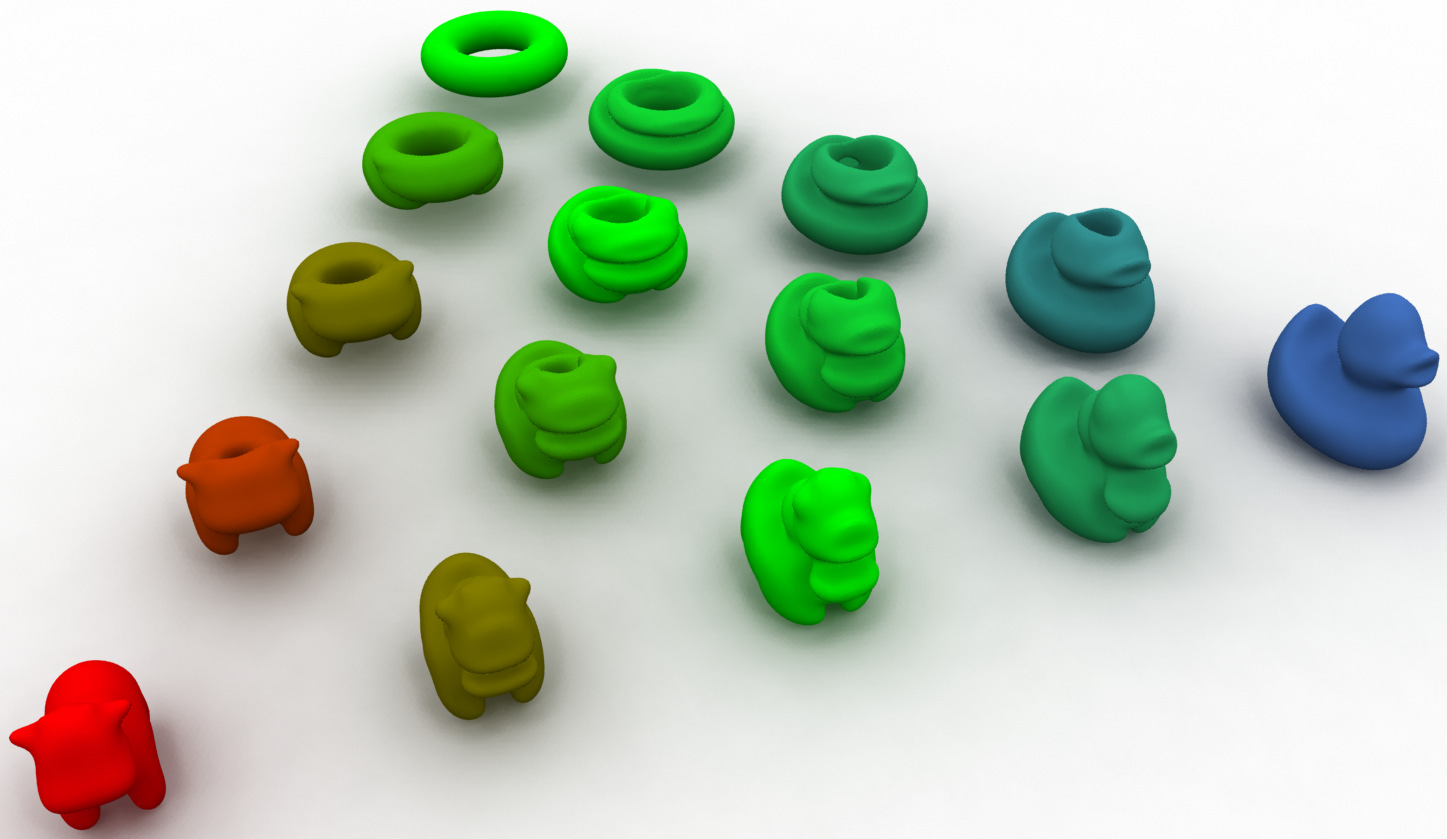
\includegraphics[scale=0.22]{shape_int.png}
			\caption{Application to shape interpolation}
			\label{shape}
		\end{figure}
	\item BRDF design
	\item Color histogram manipulation
	\item Skeleton layout
	\item Soft maps
\end{itemize}
Finally \figurename~\ref{barp} and \figurename~\ref{cardp} are two images of barycenters they have computed. The first one is an image where we find barycenters of four images that are in the corners. The second is an interpolation between two cards. As we tried to reproduce it in the implementation part we put them here:

\begin{figure}[h]
	\centering
	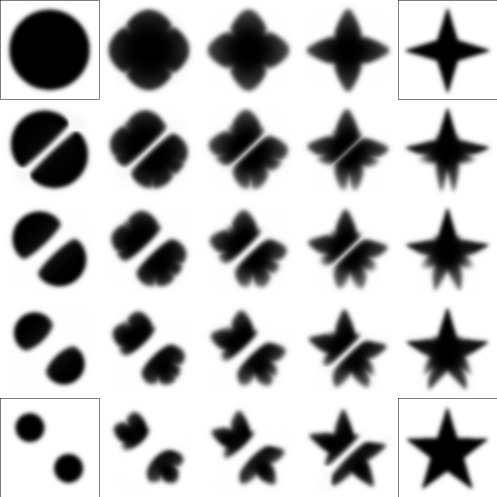
\includegraphics[scale=0.28]{bars_paper.png}
	\caption{Barycenters of four images}
	\label{barp}
\end{figure}
\begin{figure}[h]
	\centering
	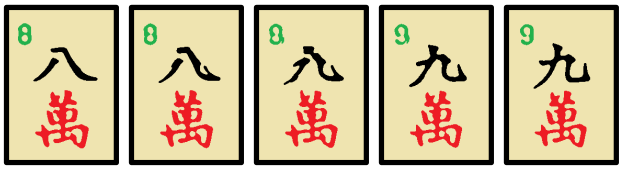
\includegraphics[scale=0.45]{cards_paper.png}
	\caption{Interpolation of two images of cards for times $t = 0, 0.25, 0.5, 0.75, 1$.}
	\label{cardp}
\end{figure}
